\documentclass{article}

% if you need to pass options to natbib, use, e.g.:
%     \PassOptionsToPackage{numbers, compress}{natbib}
% before loading neurips_2023


% ready for submission
% \usepackage{neurips_2023}


% to compile a preprint version, e.g., for submission to arXiv, add add the
% [preprint] option:
\usepackage[preprint]{neurips_2023}


% to compile a camera-ready version, add the [final] option, e.g.:
%     \usepackage[final]{neurips_2023}


% to avoid loading the natbib package, add option nonatbib:
%    \usepackage[nonatbib]{neurips_2023}


\usepackage[utf8]{inputenc} % allow utf-8 input
\usepackage[T1]{fontenc}    % use 8-bit T1 fonts
\usepackage{hyperref}       % hyperlinks
\usepackage{url}            % simple URL typesetting
\usepackage{booktabs}       % professional-quality tables
\usepackage{amsfonts}       % blackboard math symbols
\usepackage{nicefrac}       % compact symbols for 1/2, etc.
\usepackage{microtype}      % microtypography
\usepackage{xcolor}         % colors
\usepackage{graphicx}
\usepackage{natbib}
\usepackage[affil-it]{authblk}
\usepackage{amsmath}

\renewcommand\Authsep{, }
\renewcommand\Authands{, }
\renewcommand\Authand{, }

\title{Multi-ContrastiveVAE disentangles perturbation effects in single cell images from pooled optical screens}


% The \author macro works with any number of authors. There are two commands
% used to separate the names and addresses of multiple authors: \And and \AND.
%
% Using \And between authors leaves it to LaTeX to determine where to break the
% lines. Using \AND forces a line break at that point. So, if LaTeX puts 3 of 4
% authors names on the first line, and the last on the second line, try using
% \AND instead of \And before the third author name.


\author[1]{\textbf{Zitong Jerry Wang}}
\author[2]{\textbf{Romain Lopez}}
  % \texttt{zwang2@caltech.edu} }
  % examples of more authors
\author[2]{\textbf{Jan-Christian Hütter}}
\author[2]{\textbf{Takamasa Kudo}}
\author[2]{\textbf{Heming Yao}}
\author[2]{\textbf{Philipp Haslovsky}}
% could help with posting open source code / preprocessing / releasing
\author[2]{\textbf{Burkhard Hoeckendorf}}
\author[2]{\textbf{Aviv Regev}}
\affil[1]{California Institute of Technology}
\affil[2]{Genentech Research and Early Development}


\begin{document}


\maketitle


\begin{abstract}
  
\end{abstract}


\section*{Introduction}
Large-scale, pooled genetic perturbation screens in cells enable unbiased interrogation of gene function, and spatial imaging represents a promising phenotypic read-out for characterizing perturbation effects as they are high-throughput and low-cost.

Traditional phenotype analysis requires extracting from each image a set of hand-crafted morphological features, which are inherently difficult to generalize and scale to complex datasets.
In the context of large-scale perturbations, hand-crafted features may be inflexible to capture novel morphologies that are absent from the natural cell population. Furthermore morphology varies drastically across cell types and experimental conditions, so it may be necessary to constantly engineer new features for different experiments.
Conventional tools like CellProfiler which were designed to work on images with a 2-5 channels will be difficult to scale in order to capture more complex patterns in images with tens to hundreds of channels which are becoming increasingly common.

Advances in deep learning could overcome limitations of hand-crafted features by learning representations directly from data. Variational autoencoders (VAEs) represent one powerful deep generative framework to capture latent structure in complex data distribution in an unsupervised manner. However, in the context of learning perturbation effects from images of cells, standard VAE implementations suffer from the important drawback that it can be difficult to isolate perturbation effects from natural cell-cell heterogeneity, which can exhibit much greater variation compared to the phenotypic effect of perturbations.

The contrastive analysis framework offers a potential solution to identify and isolate patterns induced by perturbation by using control data to remove natural background variations. For example, contrastive principal components analysis (cPCA) seeks to identify salient principal components in a target dataset by identifying those linear combinations of features that are enriched in that dataset relative to a background dataset, rather than those that simply have the most variance. Recently, neural network based contrastive methods have been shown to be effective at discovering nonlinear latent features enriched in one dataset relative to another.

We propose a contrastive framework for cell imaging datasets from optical pooled screens (OPS) by extending contrastive analysis to the setting of comparing multiple datasets to a reference dataset. We apply our method to a large-scale imaging dataset of over 30 million cells across >5000 genetic perturbations and show that we can better identify perturbation-specific phenotypes from cell variations that exist across perturbations compared to non-contrastive methods.
Specifically, our method effectively separates multiple sources of technical artifacts from single cell images including non-biological variations due to batch effect, uneven plating, and uneven FOV illumination. Furthermore, our method disentangles perturbation effects into separate latent spaces depending on whether the perturbation induces novel phenotypes unseen in the control cell population. Lastly, we show that comparing the embedding from the two latent spaces enables us to better identify genes with established roles in mitosis.
Our approach can be easily applied to other perturbation datasets including both drug and genetic perturbation, with highly multiplexed images. 



\section*{A contrastive analysis framework for disentangling multiple sources of variation in single cell images of optical pooled screens
}

\begin{figure}[h!]
    \centering
    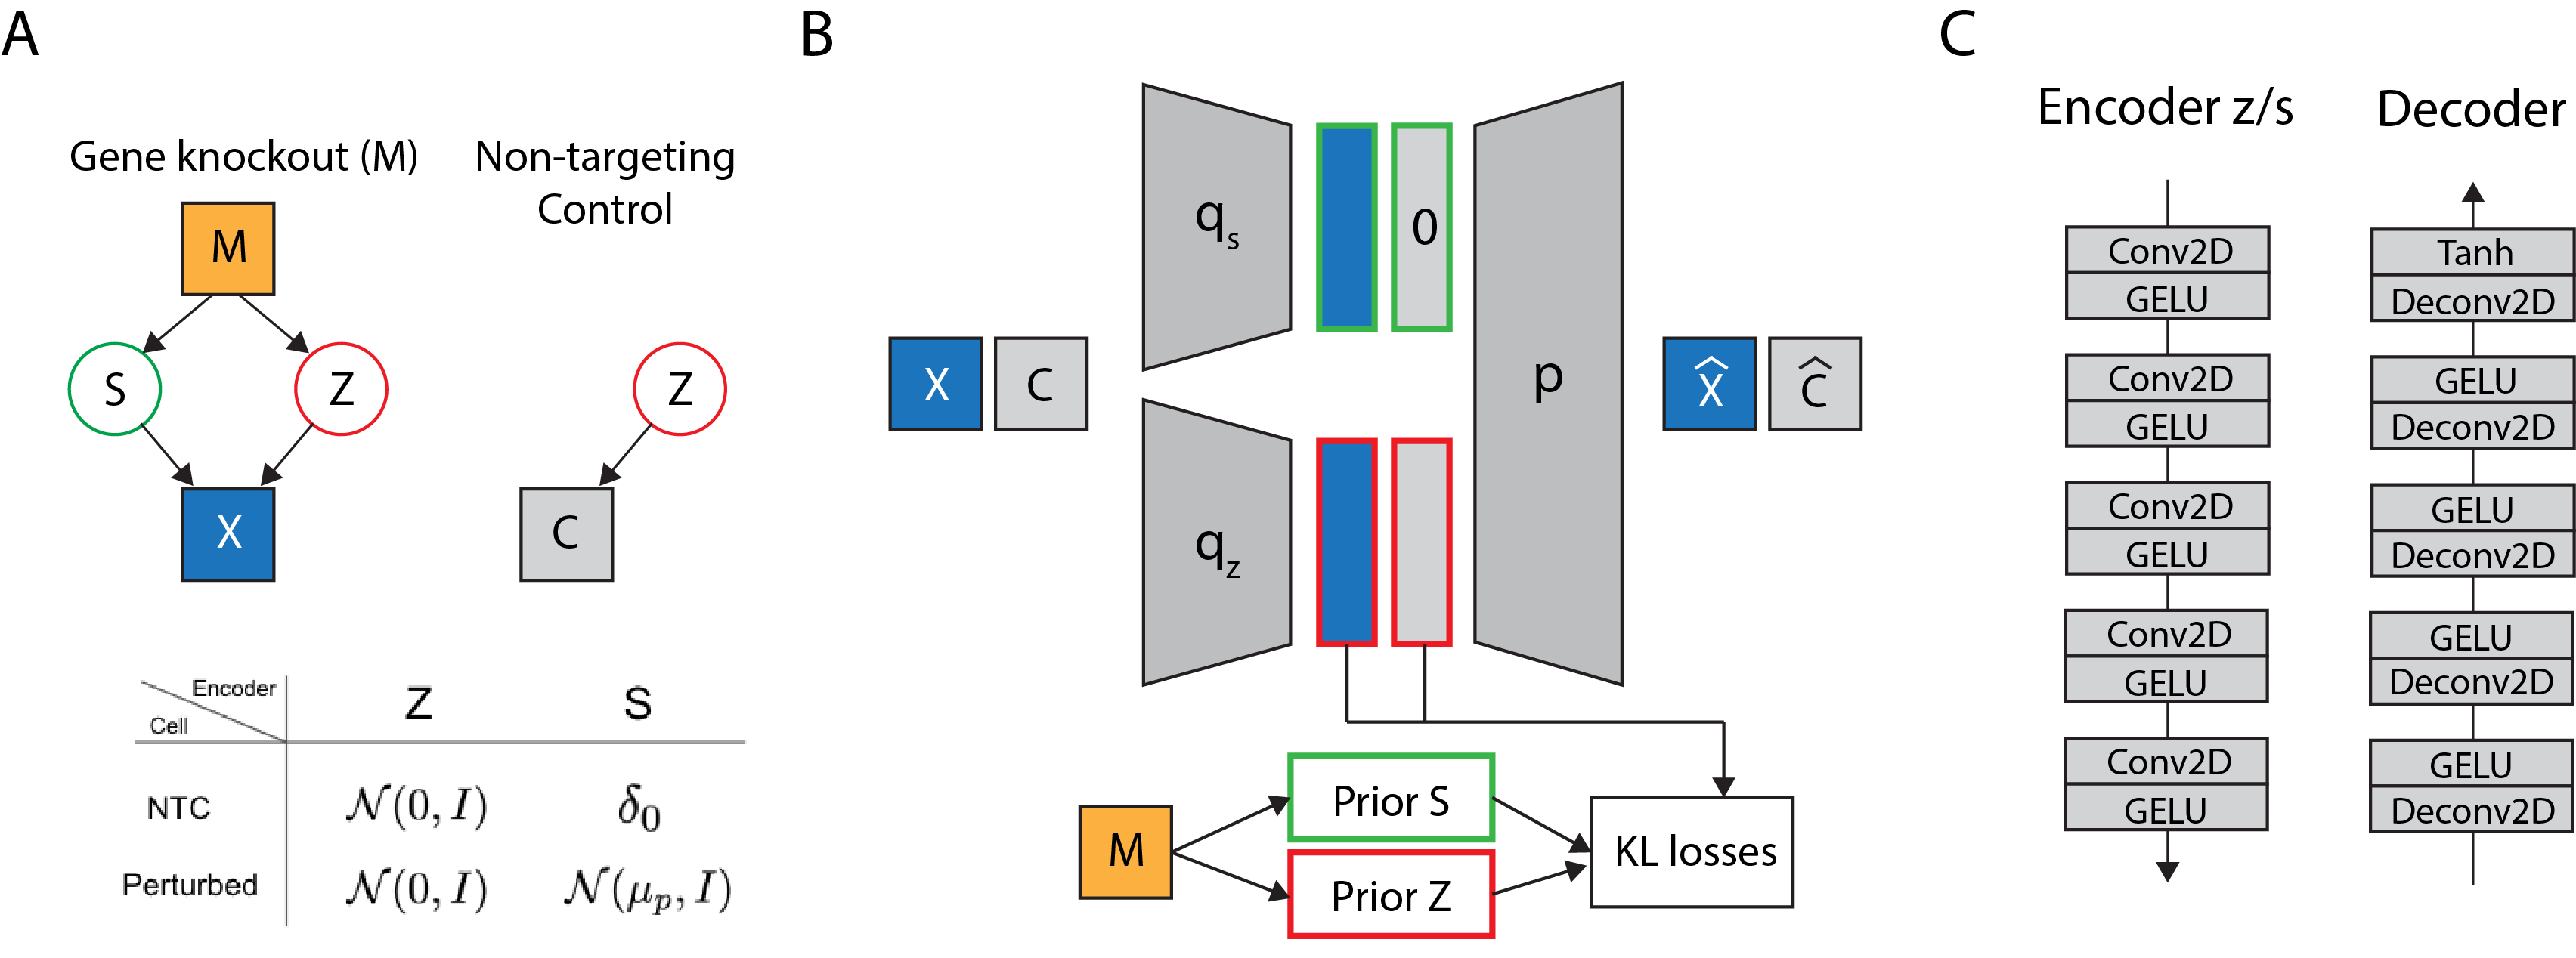
\includegraphics[width=\textwidth]{figure/figure_0.png}
    \caption{\textbf{A contrastive analysis framework for analyzing single cell images from optical pooled screen} }
    \label{fig:corum}
\end{figure}

To disentangle perturbation effects and natural cell variations in large-scale perturbation datasets, we developed Multi-Contrastive Variational Autoencoder (mcVAE) which extends the contrastive framework to the setting of comparing multiple groups to a single reference group. Our framework is built upon the work by Abid and Zou (2019), where we model perturbed cell ($X$) as generated from two sources of variation, represented by salient ($S$) and background variables ($Z$) which corresponds to variations due to perturbation and variations that naturally exist in the control cell population, respectively (Figure 1A). Since the background variables represents natural variation, the control cells ($C$) is generated entirely from this source of variation. The key modification we make to this model is by adding a perturbation variable ($M$), which influences both the salient and background variable, to capture the fact that perturbations could induce both novel phenotype which should be captured in the salient space and also shift the distribution of phenotype that already exists in natural population. This modification of the generative model represents a significant departure from the original framework where the background space was interpreted as containing only uninteresting variation while the perturbation effect resides solely within the salient space. 

Specifically, under certain independence assumption, we can derive the following ELBO for the perturbed population:

\begin{equation}
\begin{split}
& \mathcal{L}_x\left(\boldsymbol{x}_i\right) \geq \underset{q_{\phi_s}(s) q_{\phi_s}(z)}{\mathbb{E}}\left[f_\theta\left(\boldsymbol{x}_i \mid \boldsymbol{s}, \boldsymbol{z}\right)\right]
-\mathrm{KL}\left(q_{\phi_s}\left(\boldsymbol{s} \mid \boldsymbol{x}_i, \boldsymbol{m}_i\right) \| p\left(\boldsymbol{s} \mid \boldsymbol{m}_i\right)\right) \\
& -\operatorname{KL}\left(q_{\phi_z}\left(\boldsymbol{z} \mid \boldsymbol{x}_i, \boldsymbol{m}_i\right) \| p\left(\boldsymbol{z} \mid \boldsymbol{m}_i\right)\right) 
\end{split}
\end{equation}

And, we have the following ELBO for the NTCs:

\begin{equation}
\begin{split}
& \mathcal{L}_c\left(\boldsymbol{c}_i\right) \geq \underset{q_{\phi_s}(z)}{\mathbb{E}}\left[f_\theta\left(\boldsymbol{c}_i \mid \boldsymbol{0}, \boldsymbol{z}\right)\right] -\operatorname{KL}\left(q_{\phi_z}\left(\boldsymbol{z} \mid \boldsymbol{c}_i, \boldsymbol{0}\right) \| p\left(\boldsymbol{z} \mid \boldsymbol{0}\right)\right) 
\end{split}
\end{equation}

To learn the latent variables S and Z directly from data, we use two probabilistic encoders $q(s|x)$ and $q(z|x)$ to approximate the posterior of the two latent variables $s$ and $z$. The output of the two encoders are concatenated and fed into a shared decoder $p(x|s,z)$ to generate a reconstruction $\hat{x}$. We incorporate the perturbation (M) information into the model by setting the mean of the latent priors $p(s)$ and $p(z)$ as separate functions of the perturbation label. 

Since we are applying our framework to imaging data, we use simple convolutional architecture for both the encoder and decoder. Specifically, the encoder consists of five convolutional layers and the decoder consists of five transpose-convolutional layers. 

We apply our framework to a public dataset of a large-scale CRISPR-knockout screen, consisting of 30 million cells across over 5,000 genetic perturbations. We assess how well the embedding from our mcVAE reflect known biology, how well it isolates for technical artifacts, and how the salient and background space differ in terms of the perturbation effects they capture. 

\section*{Multi-Contrastive VAE outperforms Contrastive VAE and matches CellProfiler on CORUM identification
}


\begin{figure}[h!]
    \centering
    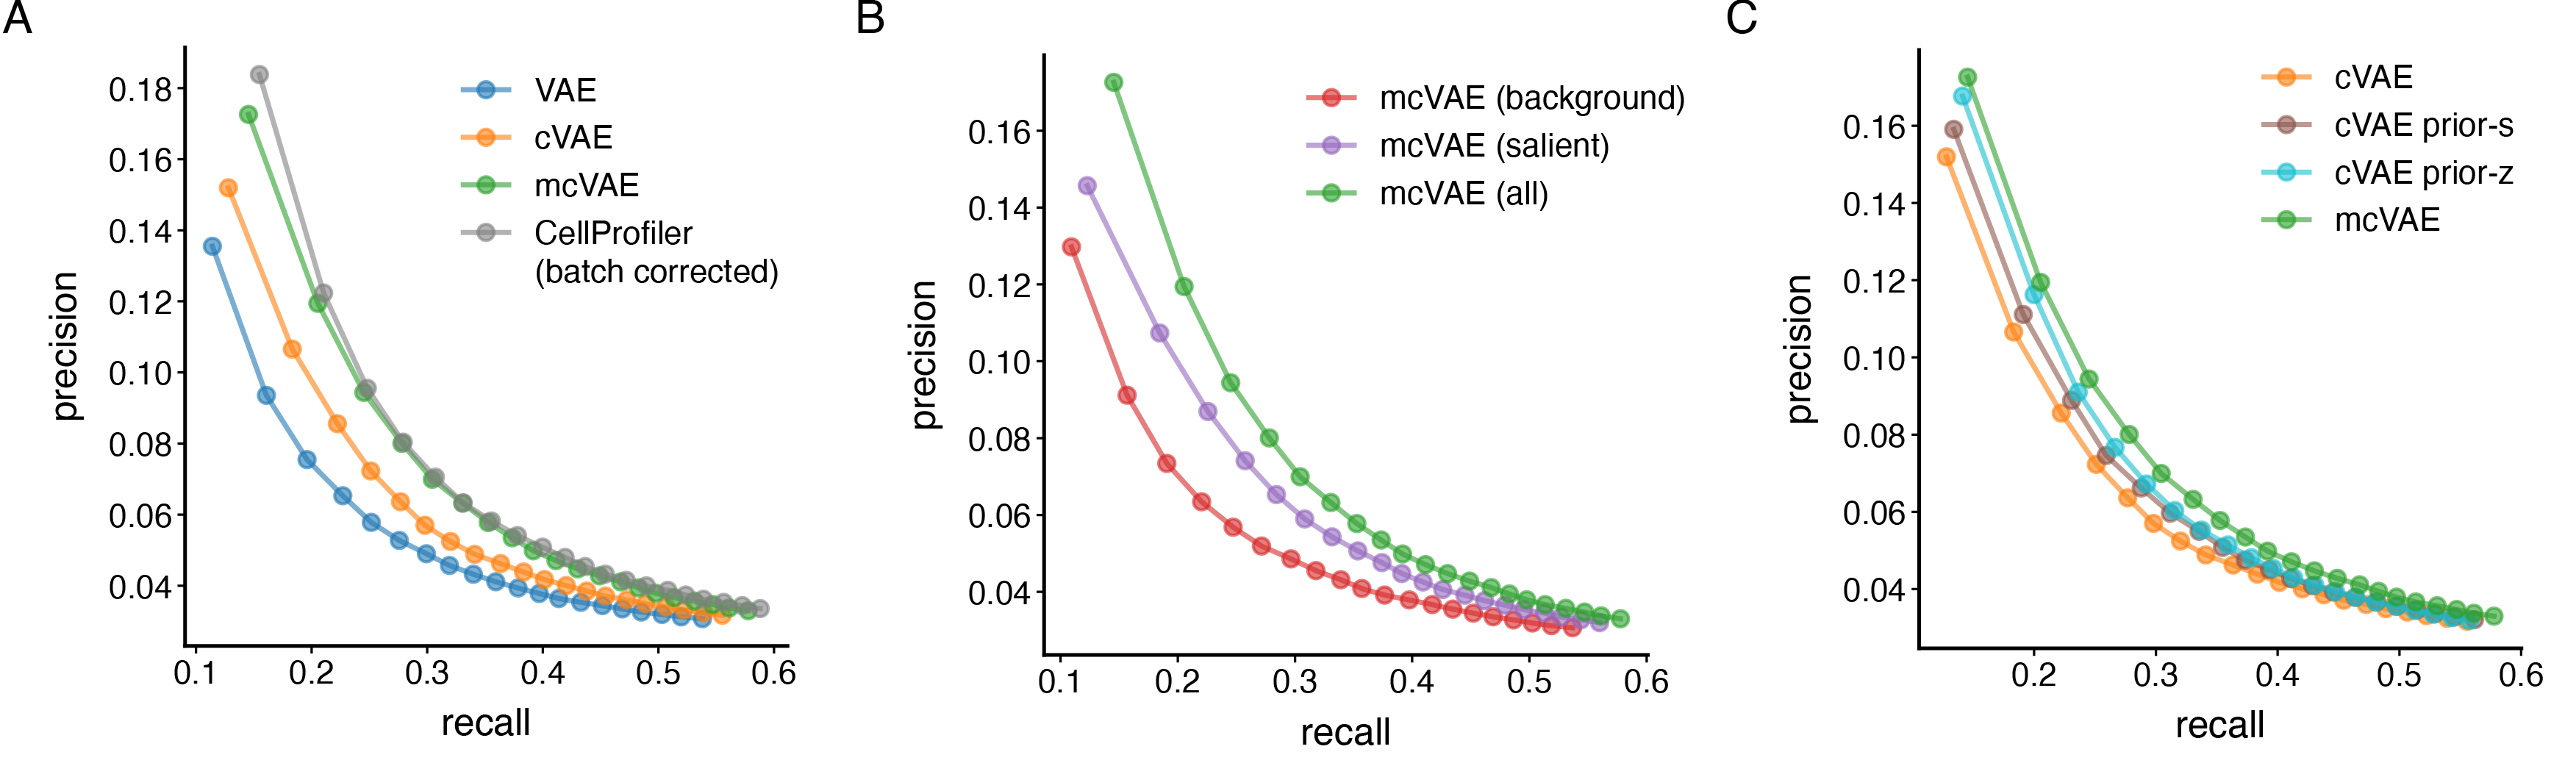
\includegraphics[width=\textwidth]{figure/figure_1.png}
    \caption{\textbf{Multi-Contrastive VAE outperforms contrastiveVAE in protein complex identification} 
    A) Precision-recall curve for CORUM identification task for vanilla VAE, contrastiveVAE (cVAE), multi-contrastiveVAE (mcVAE) and using CellProfiler features.
    B) Precision-recall curve when using background alone, salient alone, or a concatenation of both sets of latent variable.
    C) Precision-recall curve for cVAE, cVAE with perturbation label fed into just the salient prior, cVAE with perturbation label fed into just the background prior, and our mcVAE where perturbation labels are fed into both the salient and background prior}
    \label{fig:corum}
\end{figure}


We evaluated the effectiveness of our learned embeddings in capturing known biological structures by employing them to predict established protein complexes. Given that perturbations to different subunits of a complex are likely to generate analogous cellular phenotypes, it is reasonable to expect the images corresponding to these perturbations to be proximate within the embedding space.

To conduct this assessment, we utilized the CORUM database, the most extensive publicly available collection of manually curated mammalian protein complexes. By performing a nearest-neighbor search on our image embeddings (aggregated at the gene level), we aimed to predict known interactions between protein complexes.

For each gene in the study, we classified an edge to the adjacent genes, where the edge symbolizes complex interaction. We subsequently analyzed the precision-recall curve to evaluate the classification performance of various methods.

Traditional Variational Autoencoder (VAE) was found to have the least satisfactory performance, as illustrated in \autoref{fig:corum}A. In contrast, the contrastive VAE provided a substantial improvement. Our proposed model, the multi-contrastive VAE, conferred an additional significant enhancement, almost equating the boost observed in progressing from the vanilla VAE to the contrastive variant, thereby matching the performance of CellProfiler. Here we do not use all of the CellProfiler features, instead we first perform PCA at the cell-level and then take the first 64 PCs (77\% variance explained) in order to match the latent dimension of our combined salient and background space.

%should we also add comparison to the case of only changing s prior and only changing z prior? 

Furthermore, \autoref{fig:corum}B reveals that the background embedding is replete with biological information. Interestingly, the best performance for CORUM identifiability was not achieved by discarding the background information; instead, it was attained by concatenating the salient features with the background. Thus it is not surprising when we remove either the label information from the salient prior or the background prior, we obtain sub-optimal performance (\autoref{fig:corum}C). These findings emphasize the critical role of both the salient and background latent variables play in identifying protein complex interactions, and highlights the strength of our multi-contrastive VAE approach in elucidating complex biological relationships.

\section*{Multi-ContrastiveVAE disentangles multiple sources of technical artifacts from single cell images
}

\begin{figure}[h!]
    \centering
    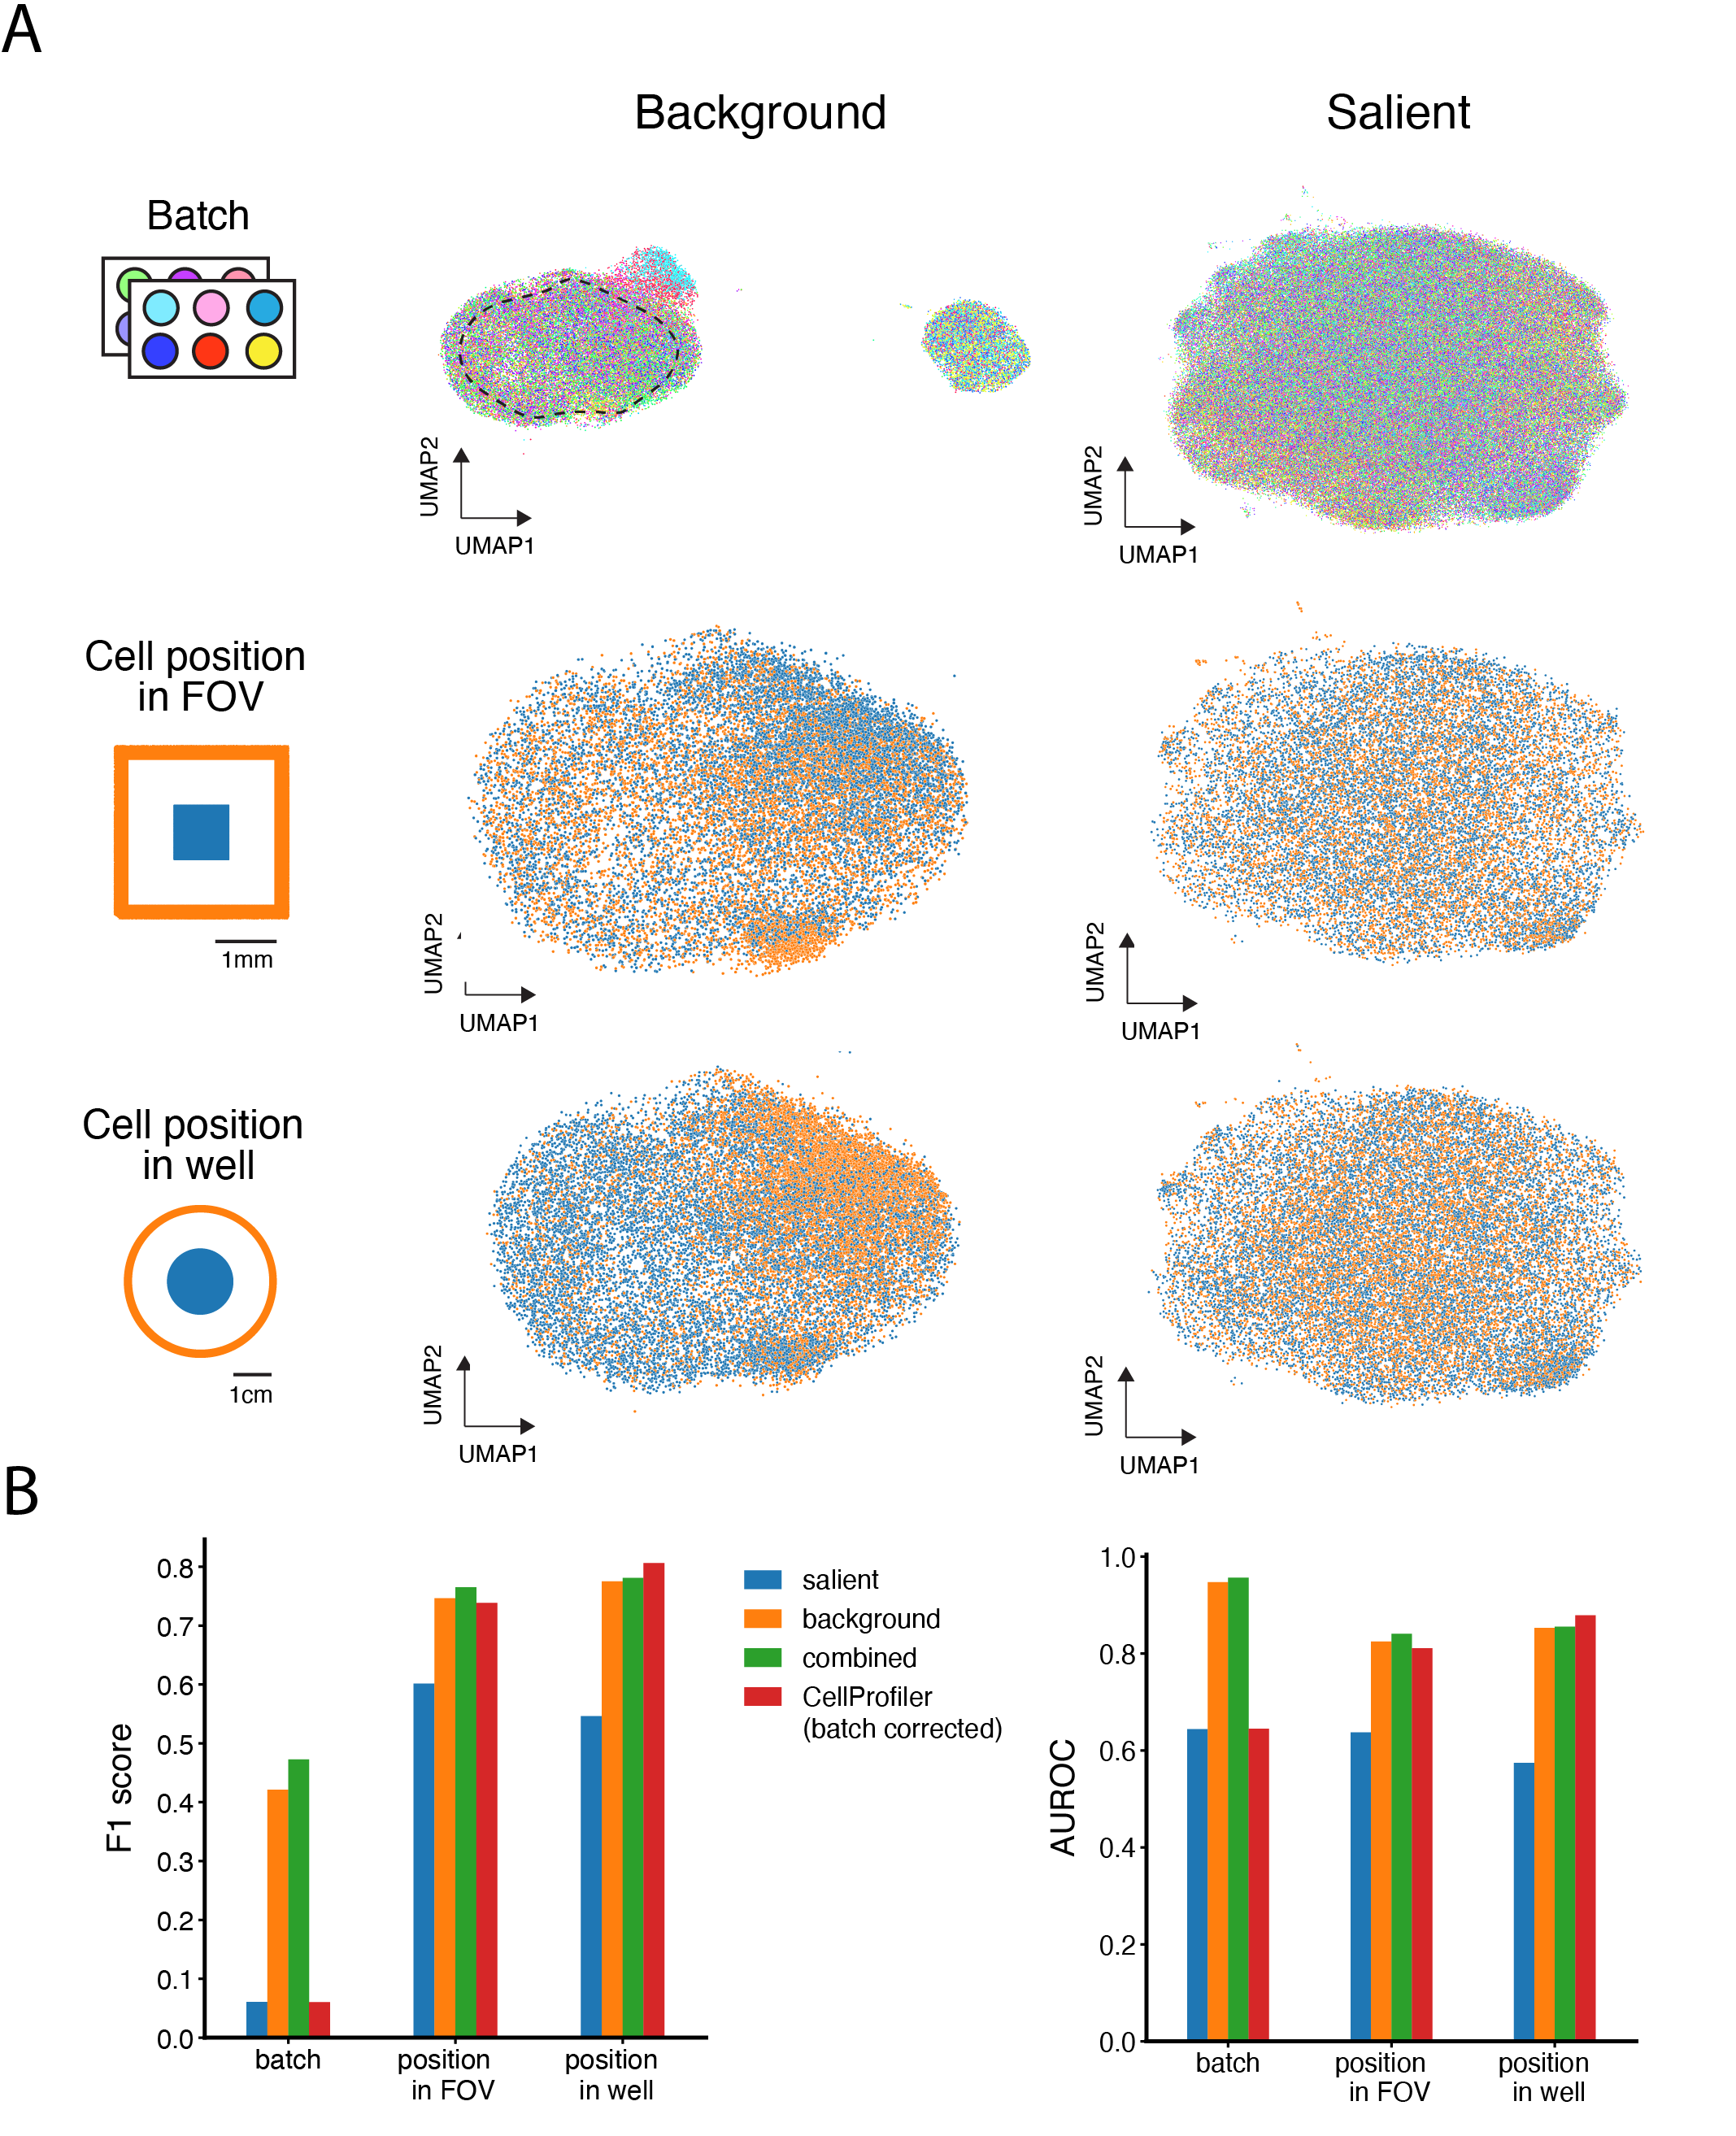
\includegraphics[width=\textwidth]{figure/figure_2.png}
    \caption{\textbf{Multiple experimental technical artifacts are found in background and CellProfiler features, while the salient space is nearly free of these artifacts}
    A) UMAP projections of background and salient embedding for individual cells colored by the batch/well they are from (top), their position in an image's field of view (edge/center), and their position in a well (cell/position). The embedding for the FOV and well position are for cells from one particular patch, outlined by dashed black line in the top left UMAP projection.
    B) Performance metrics for a logistic regression model trained to predict the three technical covariates from panel A using the cell embeddings from salient, background, salient-background combined, and batch-corrected CellProfiler.}
    \label{fig:artifact}
\end{figure}


Multi-contrastiveVAE (mcVAE) can isolate intricate technical artifacts found in cell images without any prior information on what such artifacts may be. Technical artifacts can include variations in imaging data, changes in equipment or lighting conditions, uneven illumination, or uneven seeding density of cells in a well.

mcVAE's ability to identify different technical variations is evident from the following observations. Changes in equipment or lighting can cause batch-batch variations, as shown in \autoref{fig:artifact}A (top), where background cell embeddings cluster by batch in the UMAP projection, while cells from different batches are well-mixed in the salient space. Uneven illumination of a field of view can cause cells near the center to appear brighter than those near the edge. \autoref{fig:artifact}A (middle) illustrates that background cell embeddings capture this variation, while the salient space appears well-mixed, indicating removal of this technical variation. \autoref{fig:artifact}A (bottom) reveals that background cell embeddings are separated based on their position in a well, influenced by uneven cell density affecting cell shape and size. This source of variation is absent in the salient space.

To quantify the presence of technical variation in different embedding spaces, logistic regression models were trained to predict various technical covariates from the cell embeddings. \autoref{fig:artifact}B shows that the salient embeddings are most free of technical artifacts, as evidenced by the poorest performance in both F1 score and AUROC (area under receiver operating characteristic curve).

In contrast, both the background and CellProfiler embeddings contain significant technical variations in terms of FOV position and well position. The CellProfiler embedding used was batch-corrected (by standardizing against the NTC in the corresponding batch), effective at removing batch effects but unable to address the other two, more intricate sources of technical variations.


\section*{Background and salient space excel at predicting different functional groups of genes based on whether the perturbation induce novel phenotypes}


\begin{figure}[h!]
    \centering
    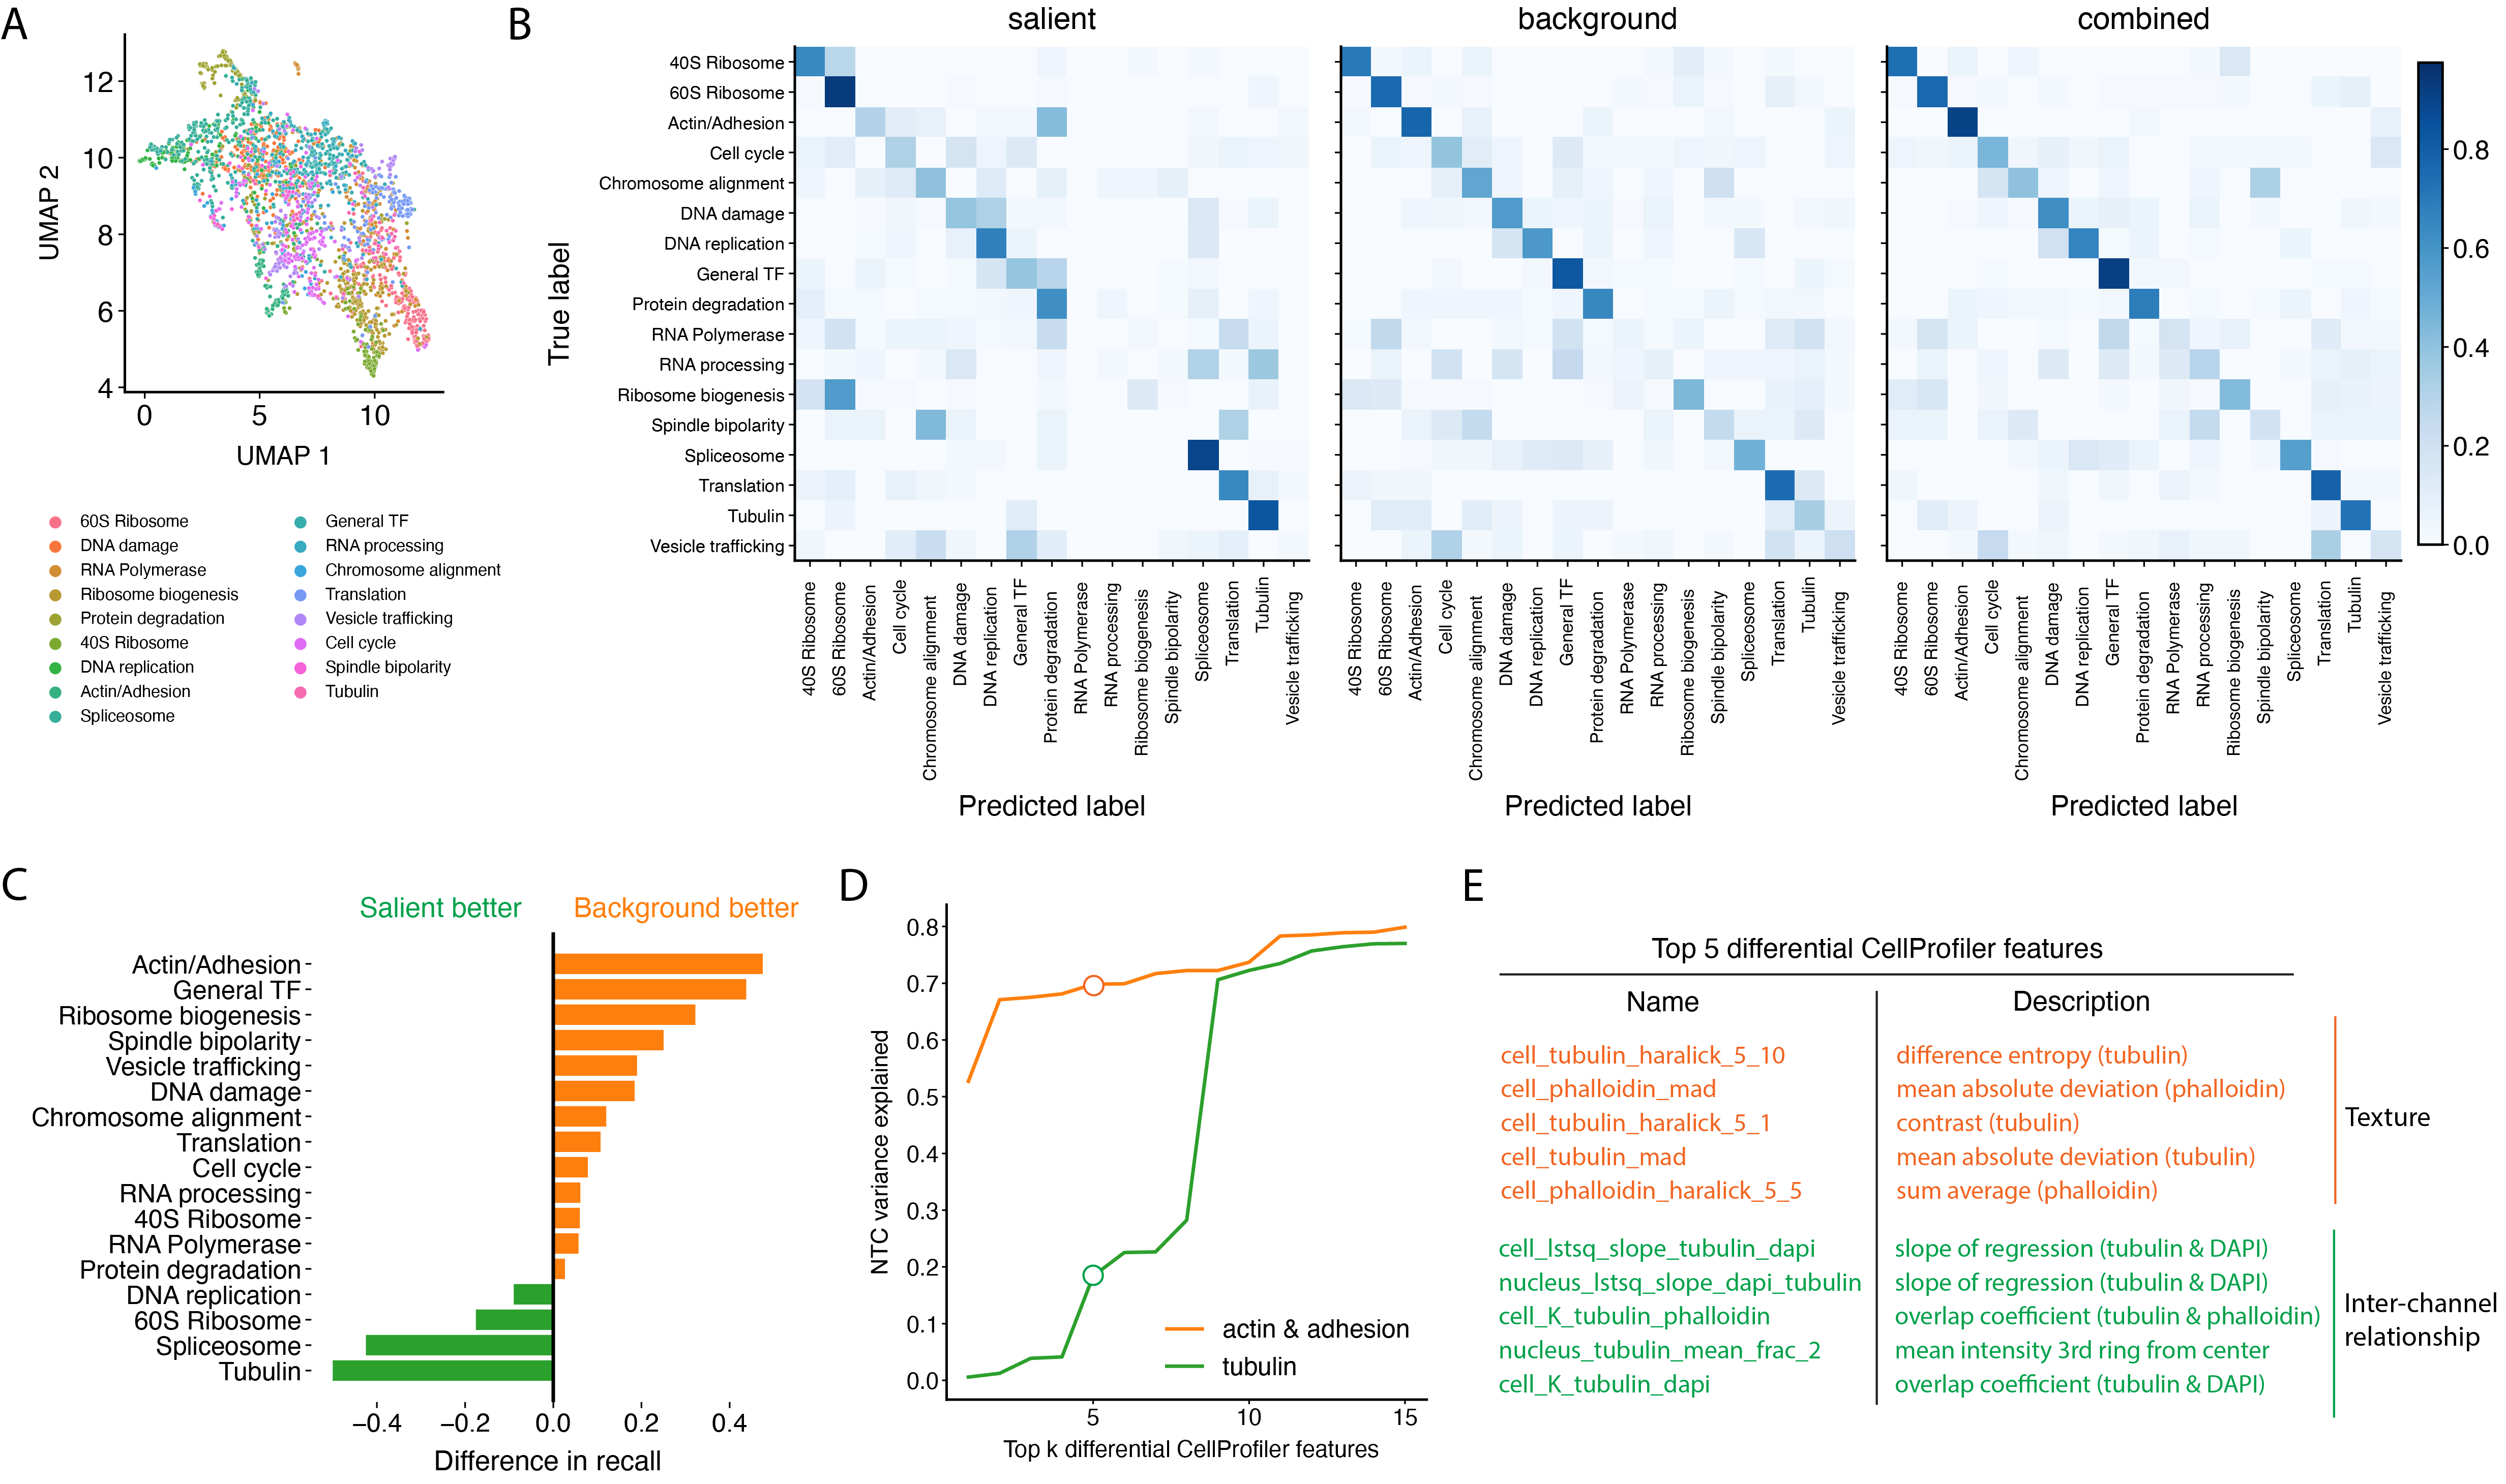
\includegraphics[width=\textwidth]{figure/figure_3.png}
    \caption{\textbf{Salient space better predicts perturbation that induces novel phenotype while background space better predicts perturbation that changes the distribution of existing phenotype}
    A) .
    B) .
    C) .
    D) .
    E) .}
    \label{fig:genefunction}
\end{figure}


Both salient and background embedding can be used to accurately classify gene functions, albeit with significant differences in performance depending on the particular functional group. The process of assessment began with aggregating cells to the level of CRISPR guides and training a logistic regression model to classify the function of the perturbed gene into one of 17 pre-defined functional groups. \autoref{fig:genefunction}A presents a UMAP projection of guide embedding in the combined salient-background space, showing that genes of the same functional groups tend to cluster together. This clustering suggests that the embedding space is rich in biological information.

From the confusion matrix in \autoref{fig:genefunction}B, generated using our trained linear classifier, we observe that the combined embedding performs the best compared to using either the salient or background embedding separately. However, it's important to note that the classification performance of the salient and background space can vary significantly depending on the function group, and also when compared to each other. \autoref{fig:genefunction}C provides a visualization of these differences in terms of recall between classifiers trained on background versus salient embedding. Specific variations were identified, where background embedding excels at predicting gene functional groups such as actin cytoskeleton/adhesion, spindle bipolarity, DNA damage, and chromosome alignment, while salient embedding is more efficient at predicting genes associated with tubulin and spliceosome.

We sought to understand the cause of this difference between background and salient embedding. We reason that perturbing genes associated with certain functions that would likely affect phenotype associated with cell shape and cell cycle stage, phenotype variations that are primarily captured by the background space. Conversely, perturbing genes in the tubulin group generates features that see less variation in non-targeting control cells (NTCs). To test this hypothesis, we performed multiple hypothesis testing to identify the top CellProfiler features altered by genetic perturbation and measured how much variation in NTCs can be explained by these altered features.

\autoref{fig:genefunction}D reveals significant insights: cell features perturbed by knocking out genes in the actin \& adhesion group can explain substantially more variation in the first principle component of NTCs compared to using features altered by knocking out genes in the tubulin group. Specifically, using the top altered feature from the actin \& adhesion perturbations, we can explain over 50\% of the variation in the NTC's first PC, whereas the tubulin features can barely explain any variation. Similarly, nearly 70\% of the variation can be explained when using the actin \& adhesion features but only 20\% when using the tubulin features. The features most significantly altered by perturbations to genes in the actin \& adhesion group are mainly associated with spatial heterogeneity of tubulin and actin, while features altered by tubulin-associated gene perturbations relate to correlation and overlap between tubulin and other molecular structures, explaining less of the variations in NTCs. 

The section illustrates that the differences in classification performance between salient and background embedding stem from the nature of the gene perturbations, specifically whether they generate new phenotypes or merely shift the distribution of existing phenotypes, shedding light on the complex interaction between gene functions and their visual representation in the cell.


\section*{Comparing background and salient embedding enables us to identify mitotic factors}

\begin{figure}[h!]
    \centering
    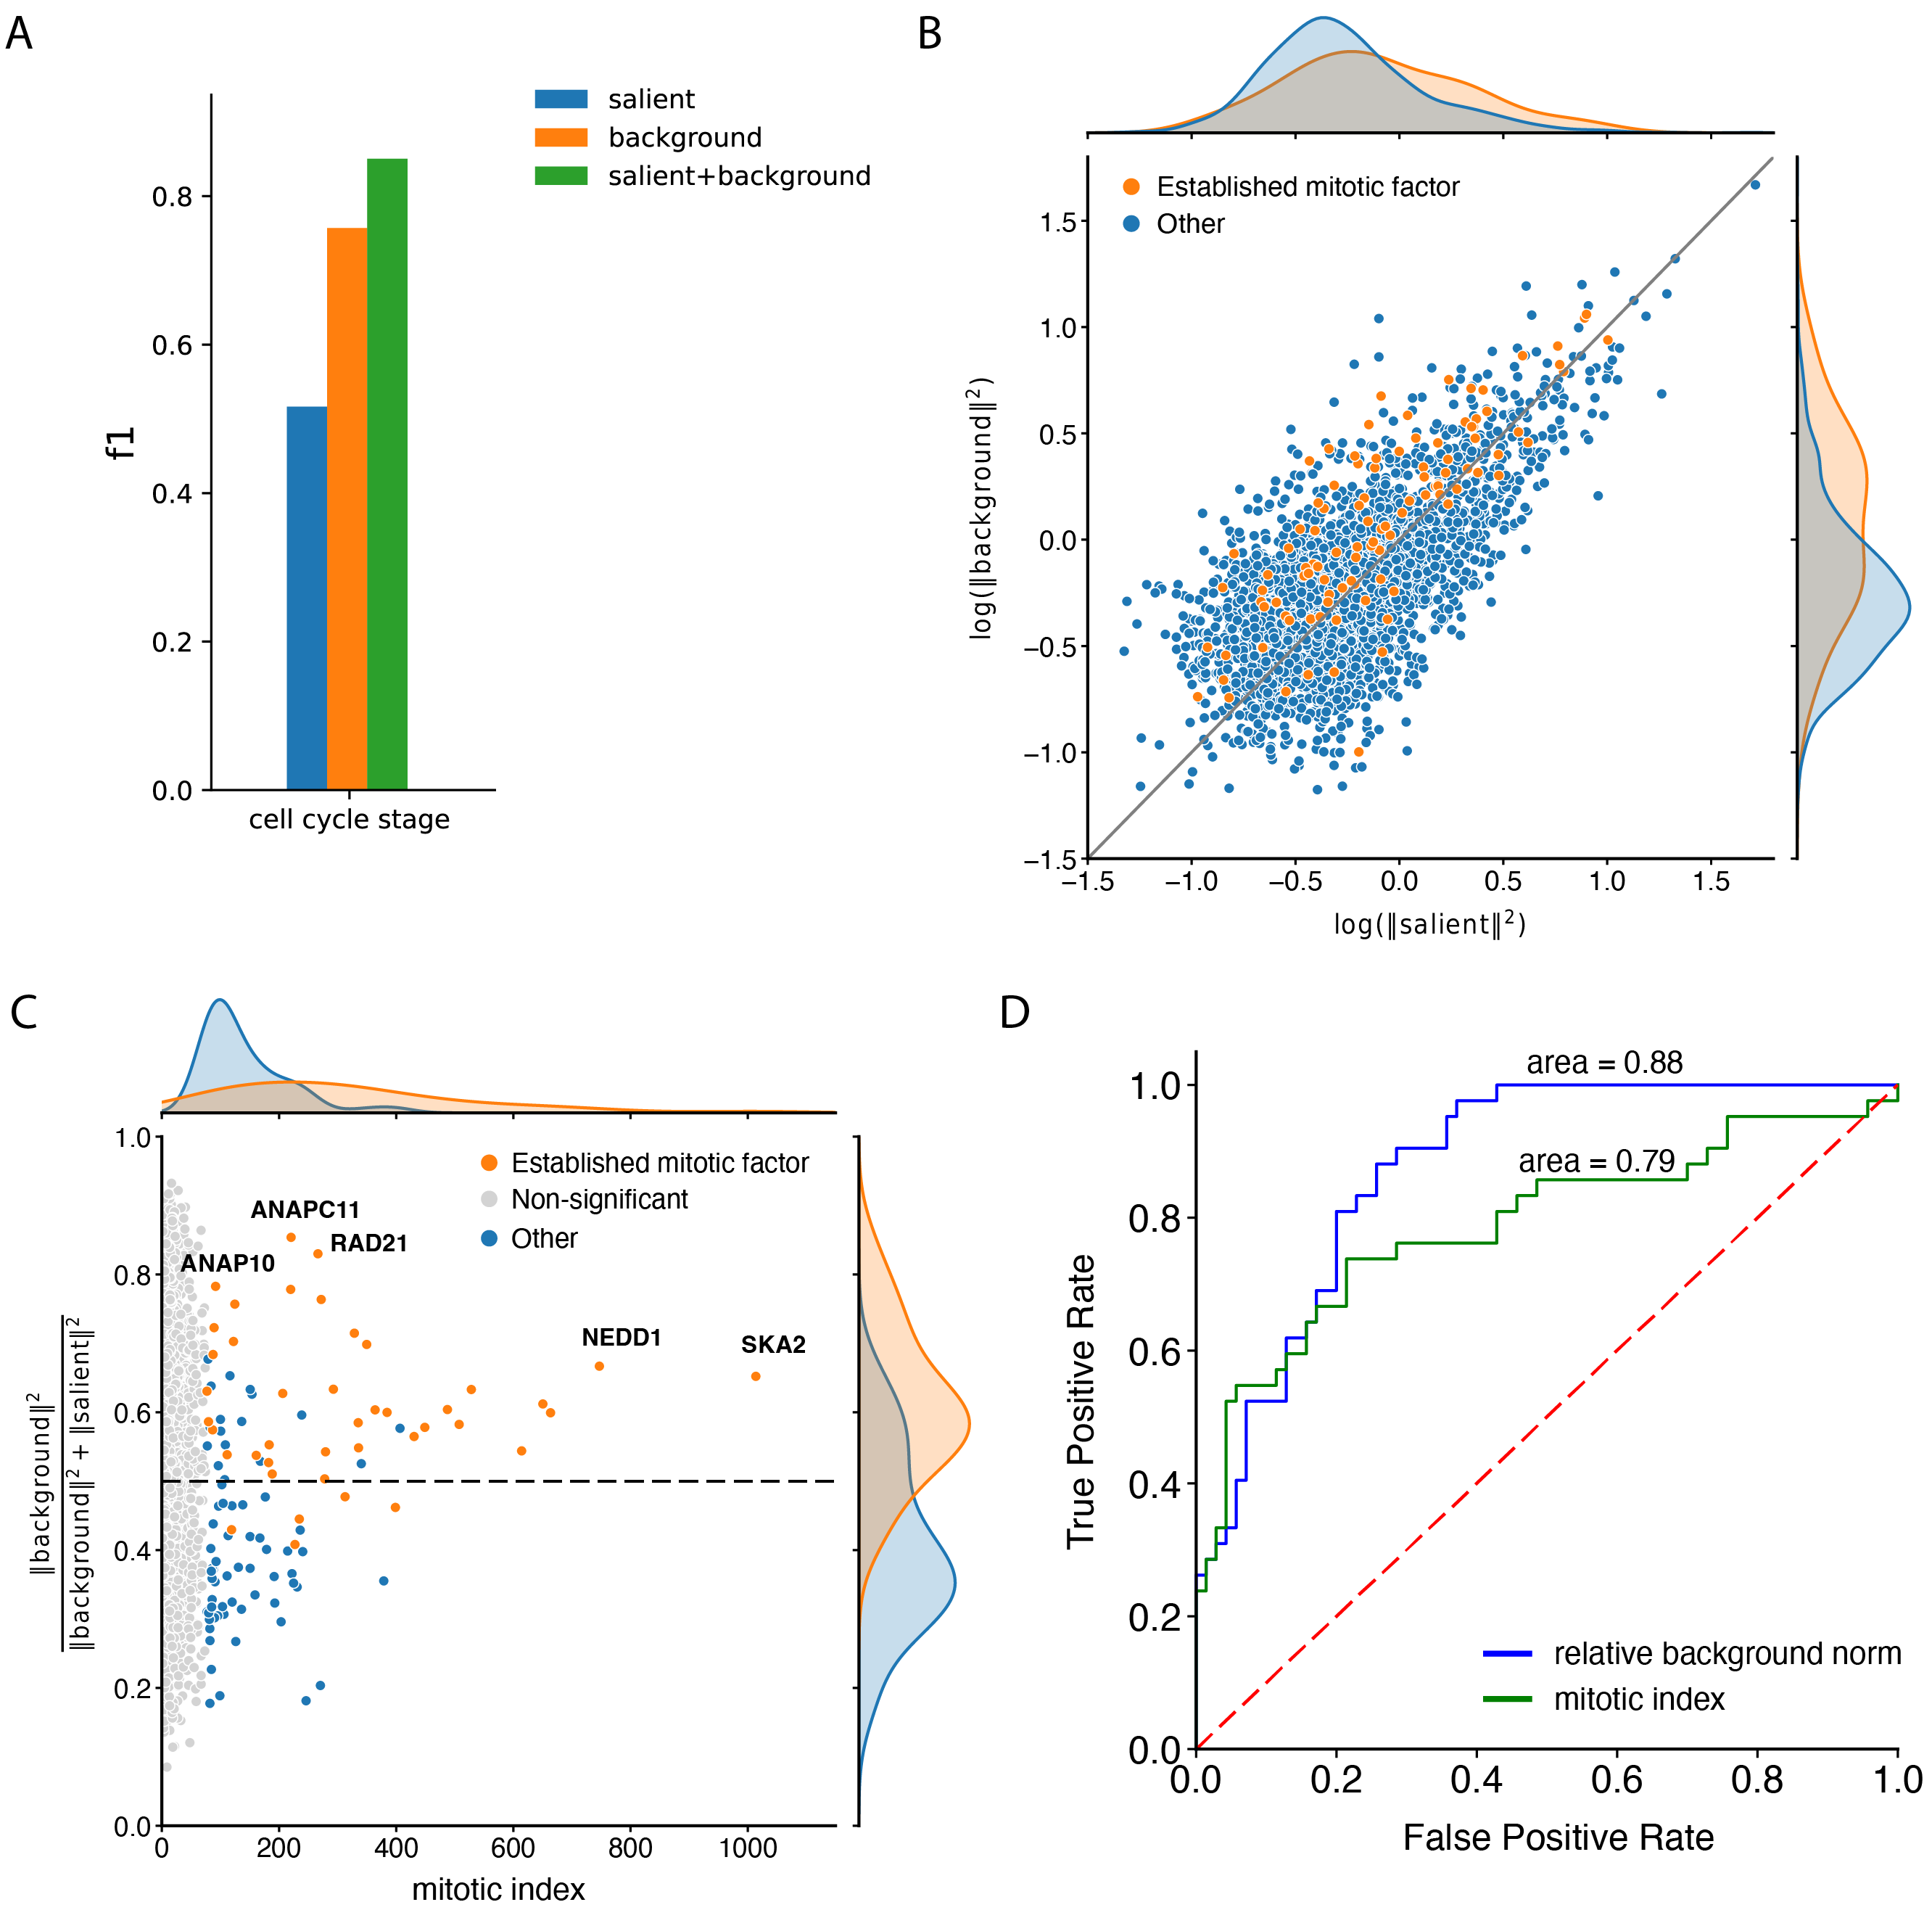
\includegraphics[width=\textwidth]{figure/figure_4.png}
    \caption{\textbf{distinguishing mitotic and non-mitotic factors by comparing the norm of background and salient embedding}
    A) F1 score for logistic regression model trained to classify a cell as in interphase or mitosis using different embedding spaces.
    B) scatterplot showing the log of background and salient embedding norms for each gene, where we have filtered to keep only genes with significant difference compared to NTCs and also normalized the salient and background embeddings to have the same norm on average across all genes.
    C) scatterplot showing mitotic index and relative background norm with a select subset of mitotic factors labeled, where significant genes (blue and orange) indicates those with a mitotic index that falls in the 99.9th percentile of NTCs).
    D) ROC curve for varying cut-off values used to classify mitotic factors, using either mitotic index or relative background norm, area denotes area under ROC curve.}
    \label{fig:mitosis}
\end{figure}

Cell cycle stage represents a strong source of phenotypic variation in a natural cell population. We can take advantage of our explicit separation of variation into background and salient space to identify factors that play an important role in mitosis. \autoref{fig:mitosis}A shows that indeed the background space captures most of the cell cycle related variations. This is illustrated by the fact that a linear classifier achieves strong performance in predicting cell cycle stage (i.e., interphase vs. mitosis) when using background compared to salient embedding.

Furthermore, we can see that established mitotic factors tend to have a larger norm for their background embedding compared to their salient embedding (\autoref{fig:mitosis}B). However, it is not the case that only established mitotic factors have larger background embedding compared to salient. This is not surprising, as we have already seen in \autoref{fig:genefunction}C that the background can comprise many different kinds of biological variations beyond cell cycle.

To identify mitotic factors, we first filter out gene perturbations that do not produce significant changes in the proportion of mitotic cells compared to NTCs, defined as the mitotic index in \autoref{fig:mitosis}C. After filtering, \autoref{fig:mitosis}C shows that the relative background norm becomes highly predictive of whether a gene is a mitotic factor. In fact, in terms of AUROC score, \autoref{fig:mitosis}D shows that we can achieve better classification performance for mitotic factors using the relative background norm instead of the commonly used metric of mitotic index.


\begin{ack}

\end{ack}



\section{Supplementary Material}


\subsection*{Data acquisition and preprocessing}
% Unless otherwise stated in the paper, we performed PCA on cell-level CellProfiler features and took the first 64 PCs to match our model's latent dimension for downstream analysis.
CellProfiler features with corresponding metadata for each cell were obtained directly from the online repository Harvard Dataverse \citep{DVN/VYKTI5_2022}. These features were already batch-corrected by standardizing against the NTCs in the corresponding batch. 

Raw microscopy images each covering a large field of view with many cells were downloaded from BioImage Archive \citep{LukeFunk2022}, followed by imaging channel alignment using phase cross-correlation. For each raw image, pixels with intensity values in the top and bottom 0.1\% were clipped. Finally we obtain individual cell patches by using the cell positional values from CellProfiler data to obtain a 100 pixel by 100 pixel bounding box around each cell which we use to represent individual cells for model training, this also led us to drop cells within 50 pixel of the tile edge.


\vskip 0.2in

\bibliographystyle{plainnat} 
\bibliography{bibliography}

%%%%%%%%%%%%%%%%%%%%%%%%%%%%%%%%%%%%%%%%%%%%%%%%%%%%%%%%%%%%


\end{document}